% Created by tikzDevice version 0.12.3.1 on 2021-07-04 22:50:57
% !TEX encoding = UTF-8 Unicode
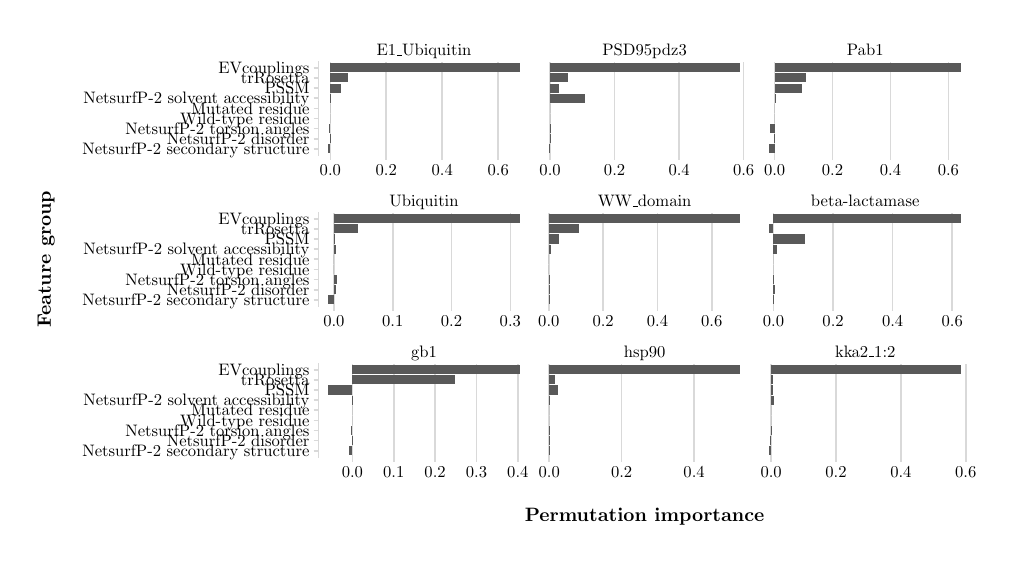
\begin{tikzpicture}[x=1pt,y=1pt]
\definecolor{fillColor}{RGB}{255,255,255}
\path[use as bounding box,fill=fillColor,fill opacity=0.00] (0,0) rectangle (344.26,183.39);
\begin{scope}
\path[clip] (105.09,137.39) rectangle (181.31,171.09);
\definecolor{drawColor}{gray}{0.85}

\path[draw=drawColor,line width= 0.6pt,line join=round] (109.37,137.39) --
	(109.37,171.09);

\path[draw=drawColor,line width= 0.6pt,line join=round] (129.59,137.39) --
	(129.59,171.09);

\path[draw=drawColor,line width= 0.6pt,line join=round] (149.81,137.39) --
	(149.81,171.09);

\path[draw=drawColor,line width= 0.6pt,line join=round] (170.03,137.39) --
	(170.03,171.09);
\definecolor{fillColor}{gray}{0.35}

\path[fill=fillColor] (109.37,163.58) rectangle (115.82,166.88);

\path[fill=fillColor] (109.37,159.92) rectangle (113.23,163.21);

\path[fill=fillColor] (109.17,156.25) rectangle (109.37,159.55);

\path[fill=fillColor] (108.55,137.94) rectangle (109.37,141.24);

\path[fill=fillColor] (109.33,141.60) rectangle (109.37,144.90);

\path[fill=fillColor] (108.71,145.27) rectangle (109.37,148.56);

\path[fill=fillColor] (109.37,167.24) rectangle (177.85,170.54);

\path[fill=fillColor] (109.37,148.93) rectangle (109.37,152.23);

\path[fill=fillColor] (109.37,152.59) rectangle (109.37,155.89);
\end{scope}
\begin{scope}
\path[clip] (105.09, 82.85) rectangle (181.31,116.54);
\definecolor{drawColor}{gray}{0.85}

\path[draw=drawColor,line width= 0.6pt,line join=round] (110.65, 82.85) --
	(110.65,116.54);

\path[draw=drawColor,line width= 0.6pt,line join=round] (131.90, 82.85) --
	(131.90,116.54);

\path[draw=drawColor,line width= 0.6pt,line join=round] (153.16, 82.85) --
	(153.16,116.54);

\path[draw=drawColor,line width= 0.6pt,line join=round] (174.41, 82.85) --
	(174.41,116.54);
\definecolor{fillColor}{gray}{0.35}

\path[fill=fillColor] (110.65,109.04) rectangle (119.28,112.33);

\path[fill=fillColor] (110.65,105.37) rectangle (110.66,108.67);

\path[fill=fillColor] (110.65,101.71) rectangle (111.52,105.01);

\path[fill=fillColor] (108.55, 83.40) rectangle (110.65, 86.69);

\path[fill=fillColor] (110.65, 87.06) rectangle (111.35, 90.36);

\path[fill=fillColor] (110.65, 90.72) rectangle (111.73, 94.02);

\path[fill=fillColor] (110.65,112.70) rectangle (177.85,115.99);

\path[fill=fillColor] (110.65, 94.39) rectangle (110.65, 97.68);

\path[fill=fillColor] (110.65, 98.05) rectangle (110.65,101.34);
\end{scope}
\begin{scope}
\path[clip] (105.09, 28.30) rectangle (181.31, 62.00);
\definecolor{drawColor}{gray}{0.85}

\path[draw=drawColor,line width= 0.6pt,line join=round] (117.33, 28.30) --
	(117.33, 62.00);

\path[draw=drawColor,line width= 0.6pt,line join=round] (132.27, 28.30) --
	(132.27, 62.00);

\path[draw=drawColor,line width= 0.6pt,line join=round] (147.22, 28.30) --
	(147.22, 62.00);

\path[draw=drawColor,line width= 0.6pt,line join=round] (162.17, 28.30) --
	(162.17, 62.00);

\path[draw=drawColor,line width= 0.6pt,line join=round] (177.12, 28.30) --
	(177.12, 62.00);
\definecolor{fillColor}{gray}{0.35}

\path[fill=fillColor] (117.33, 54.49) rectangle (154.26, 57.79);

\path[fill=fillColor] (108.55, 50.83) rectangle (117.33, 54.12);

\path[fill=fillColor] (117.33, 47.17) rectangle (117.63, 50.46);

\path[fill=fillColor] (116.00, 28.85) rectangle (117.33, 32.15);

\path[fill=fillColor] (117.25, 32.52) rectangle (117.33, 35.81);

\path[fill=fillColor] (116.98, 36.18) rectangle (117.33, 39.47);

\path[fill=fillColor] (117.33, 58.15) rectangle (177.85, 61.45);

\path[fill=fillColor] (117.33, 39.84) rectangle (117.33, 43.14);

\path[fill=fillColor] (117.33, 43.50) rectangle (117.33, 46.80);
\end{scope}
\begin{scope}
\path[clip] (184.81,137.39) rectangle (261.04,171.09);
\definecolor{drawColor}{gray}{0.85}

\path[draw=drawColor,line width= 0.6pt,line join=round] (188.77,137.39) --
	(188.77,171.09);

\path[draw=drawColor,line width= 0.6pt,line join=round] (212.08,137.39) --
	(212.08,171.09);

\path[draw=drawColor,line width= 0.6pt,line join=round] (235.40,137.39) --
	(235.40,171.09);

\path[draw=drawColor,line width= 0.6pt,line join=round] (258.71,137.39) --
	(258.71,171.09);
\definecolor{fillColor}{gray}{0.35}

\path[fill=fillColor] (188.77,163.58) rectangle (195.17,166.88);

\path[fill=fillColor] (188.77,159.92) rectangle (191.92,163.21);

\path[fill=fillColor] (188.77,156.25) rectangle (201.35,159.55);

\path[fill=fillColor] (188.28,137.94) rectangle (188.77,141.24);

\path[fill=fillColor] (188.71,141.60) rectangle (188.77,144.90);

\path[fill=fillColor] (188.76,145.27) rectangle (188.77,148.56);

\path[fill=fillColor] (188.77,167.24) rectangle (257.57,170.54);

\path[fill=fillColor] (188.77,148.93) rectangle (188.77,152.23);

\path[fill=fillColor] (188.77,152.59) rectangle (188.77,155.89);
\end{scope}
\begin{scope}
\path[clip] (184.81, 82.85) rectangle (261.04,116.54);
\definecolor{drawColor}{gray}{0.85}

\path[draw=drawColor,line width= 0.6pt,line join=round] (188.32, 82.85) --
	(188.32,116.54);

\path[draw=drawColor,line width= 0.6pt,line join=round] (207.95, 82.85) --
	(207.95,116.54);

\path[draw=drawColor,line width= 0.6pt,line join=round] (227.57, 82.85) --
	(227.57,116.54);

\path[draw=drawColor,line width= 0.6pt,line join=round] (247.19, 82.85) --
	(247.19,116.54);
\definecolor{fillColor}{gray}{0.35}

\path[fill=fillColor] (188.32,109.04) rectangle (199.37,112.33);

\path[fill=fillColor] (188.32,105.37) rectangle (191.83,108.67);

\path[fill=fillColor] (188.32,101.71) rectangle (188.93,105.01);

\path[fill=fillColor] (188.28, 83.40) rectangle (188.32, 86.69);

\path[fill=fillColor] (188.32, 87.06) rectangle (188.80, 90.36);

\path[fill=fillColor] (188.32, 90.72) rectangle (188.46, 94.02);

\path[fill=fillColor] (188.32,112.70) rectangle (257.57,115.99);

\path[fill=fillColor] (188.32, 94.39) rectangle (188.32, 97.68);

\path[fill=fillColor] (188.32, 98.05) rectangle (188.32,101.34);
\end{scope}
\begin{scope}
\path[clip] (184.81, 28.30) rectangle (261.04, 62.00);
\definecolor{drawColor}{gray}{0.85}

\path[draw=drawColor,line width= 0.6pt,line join=round] (188.46, 28.30) --
	(188.46, 62.00);

\path[draw=drawColor,line width= 0.6pt,line join=round] (214.63, 28.30) --
	(214.63, 62.00);

\path[draw=drawColor,line width= 0.6pt,line join=round] (240.81, 28.30) --
	(240.81, 62.00);
\definecolor{fillColor}{gray}{0.35}

\path[fill=fillColor] (188.46, 54.49) rectangle (190.71, 57.79);

\path[fill=fillColor] (188.46, 50.83) rectangle (191.62, 54.12);

\path[fill=fillColor] (188.46, 47.17) rectangle (188.47, 50.46);

\path[fill=fillColor] (188.28, 28.85) rectangle (188.46, 32.15);

\path[fill=fillColor] (188.46, 32.52) rectangle (188.64, 35.81);

\path[fill=fillColor] (188.46, 36.18) rectangle (188.60, 39.47);

\path[fill=fillColor] (188.46, 58.15) rectangle (257.57, 61.45);

\path[fill=fillColor] (188.46, 39.84) rectangle (188.46, 43.14);

\path[fill=fillColor] (188.46, 43.50) rectangle (188.46, 46.80);
\end{scope}
\begin{scope}
\path[clip] (264.54,137.39) rectangle (340.76,171.09);
\definecolor{drawColor}{gray}{0.85}

\path[draw=drawColor,line width= 0.6pt,line join=round] (269.92,137.39) --
	(269.92,171.09);

\path[draw=drawColor,line width= 0.6pt,line join=round] (290.84,137.39) --
	(290.84,171.09);

\path[draw=drawColor,line width= 0.6pt,line join=round] (311.77,137.39) --
	(311.77,171.09);

\path[draw=drawColor,line width= 0.6pt,line join=round] (332.69,137.39) --
	(332.69,171.09);
\definecolor{fillColor}{gray}{0.35}

\path[fill=fillColor] (269.92,163.58) rectangle (281.08,166.88);

\path[fill=fillColor] (269.92,159.92) rectangle (279.76,163.21);

\path[fill=fillColor] (269.88,156.25) rectangle (269.92,159.55);

\path[fill=fillColor] (268.00,137.94) rectangle (269.92,141.24);

\path[fill=fillColor] (269.65,141.60) rectangle (269.92,144.90);

\path[fill=fillColor] (268.25,145.27) rectangle (269.92,148.56);

\path[fill=fillColor] (269.92,167.24) rectangle (337.30,170.54);

\path[fill=fillColor] (269.92,148.93) rectangle (269.92,152.23);

\path[fill=fillColor] (269.92,152.59) rectangle (269.92,155.89);
\end{scope}
\begin{scope}
\path[clip] (264.54, 82.85) rectangle (340.76,116.54);
\definecolor{drawColor}{gray}{0.85}

\path[draw=drawColor,line width= 0.6pt,line join=round] (269.50, 82.85) --
	(269.50,116.54);

\path[draw=drawColor,line width= 0.6pt,line join=round] (291.03, 82.85) --
	(291.03,116.54);

\path[draw=drawColor,line width= 0.6pt,line join=round] (312.56, 82.85) --
	(312.56,116.54);

\path[draw=drawColor,line width= 0.6pt,line join=round] (334.09, 82.85) --
	(334.09,116.54);
\definecolor{fillColor}{gray}{0.35}

\path[fill=fillColor] (268.00,109.04) rectangle (269.50,112.33);

\path[fill=fillColor] (269.50,105.37) rectangle (280.79,108.67);

\path[fill=fillColor] (269.50,101.71) rectangle (270.67,105.01);

\path[fill=fillColor] (269.50, 83.40) rectangle (269.74, 86.69);

\path[fill=fillColor] (269.50, 87.06) rectangle (270.09, 90.36);

\path[fill=fillColor] (269.50, 90.72) rectangle (269.52, 94.02);

\path[fill=fillColor] (269.50,112.70) rectangle (337.30,115.99);

\path[fill=fillColor] (269.50, 94.39) rectangle (269.50, 97.68);

\path[fill=fillColor] (269.50, 98.05) rectangle (269.50,101.34);
\end{scope}
\begin{scope}
\path[clip] (264.54, 28.30) rectangle (340.76, 62.00);
\definecolor{drawColor}{gray}{0.85}

\path[draw=drawColor,line width= 0.6pt,line join=round] (268.67, 28.30) --
	(268.67, 62.00);

\path[draw=drawColor,line width= 0.6pt,line join=round] (292.10, 28.30) --
	(292.10, 62.00);

\path[draw=drawColor,line width= 0.6pt,line join=round] (315.53, 28.30) --
	(315.53, 62.00);

\path[draw=drawColor,line width= 0.6pt,line join=round] (338.96, 28.30) --
	(338.96, 62.00);
\definecolor{fillColor}{gray}{0.35}

\path[fill=fillColor] (268.67, 54.49) rectangle (269.30, 57.79);

\path[fill=fillColor] (268.67, 50.83) rectangle (269.34, 54.12);

\path[fill=fillColor] (268.67, 47.17) rectangle (269.58, 50.46);

\path[fill=fillColor] (268.00, 28.85) rectangle (268.67, 32.15);

\path[fill=fillColor] (268.31, 32.52) rectangle (268.67, 35.81);

\path[fill=fillColor] (268.62, 36.18) rectangle (268.67, 39.47);

\path[fill=fillColor] (268.67, 58.15) rectangle (337.30, 61.45);

\path[fill=fillColor] (268.67, 39.84) rectangle (268.67, 43.14);

\path[fill=fillColor] (268.67, 43.50) rectangle (268.67, 46.80);
\end{scope}
\begin{scope}
\path[clip] (105.09, 62.00) rectangle (181.31, 70.80);
\definecolor{drawColor}{RGB}{0,0,0}

\node[text=drawColor,anchor=base,inner sep=0pt, outer sep=0pt, scale=  0.60] at (143.20, 64.33) {gb1};
\end{scope}
\begin{scope}
\path[clip] (184.81, 62.00) rectangle (261.04, 70.80);
\definecolor{drawColor}{RGB}{0,0,0}

\node[text=drawColor,anchor=base,inner sep=0pt, outer sep=0pt, scale=  0.60] at (222.93, 64.33) {hsp90};
\end{scope}
\begin{scope}
\path[clip] (264.54, 62.00) rectangle (340.76, 70.80);
\definecolor{drawColor}{RGB}{0,0,0}

\node[text=drawColor,anchor=base,inner sep=0pt, outer sep=0pt, scale=  0.60] at (302.65, 64.33) {kka2\_1:2};
\end{scope}
\begin{scope}
\path[clip] (105.09,116.54) rectangle (181.31,125.34);
\definecolor{drawColor}{RGB}{0,0,0}

\node[text=drawColor,anchor=base,inner sep=0pt, outer sep=0pt, scale=  0.60] at (143.20,118.88) {Ubiquitin};
\end{scope}
\begin{scope}
\path[clip] (184.81,116.54) rectangle (261.04,125.34);
\definecolor{drawColor}{RGB}{0,0,0}

\node[text=drawColor,anchor=base,inner sep=0pt, outer sep=0pt, scale=  0.60] at (222.93,118.88) {WW\_domain};
\end{scope}
\begin{scope}
\path[clip] (264.54,116.54) rectangle (340.76,125.34);
\definecolor{drawColor}{RGB}{0,0,0}

\node[text=drawColor,anchor=base,inner sep=0pt, outer sep=0pt, scale=  0.60] at (302.65,118.88) {beta-lactamase};
\end{scope}
\begin{scope}
\path[clip] (105.09,171.09) rectangle (181.31,179.89);
\definecolor{drawColor}{RGB}{0,0,0}

\node[text=drawColor,anchor=base,inner sep=0pt, outer sep=0pt, scale=  0.60] at (143.20,173.42) {E1\_Ubiquitin};
\end{scope}
\begin{scope}
\path[clip] (184.81,171.09) rectangle (261.04,179.89);
\definecolor{drawColor}{RGB}{0,0,0}

\node[text=drawColor,anchor=base,inner sep=0pt, outer sep=0pt, scale=  0.60] at (222.93,173.42) {PSD95pdz3};
\end{scope}
\begin{scope}
\path[clip] (264.54,171.09) rectangle (340.76,179.89);
\definecolor{drawColor}{RGB}{0,0,0}

\node[text=drawColor,anchor=base,inner sep=0pt, outer sep=0pt, scale=  0.60] at (302.65,173.42) {Pab1};
\end{scope}
\begin{scope}
\path[clip] (  0.00,  0.00) rectangle (344.26,183.39);
\definecolor{drawColor}{gray}{0.85}

\path[draw=drawColor,line width= 0.6pt,line join=round] (117.33, 26.55) --
	(117.33, 28.30);

\path[draw=drawColor,line width= 0.6pt,line join=round] (132.27, 26.55) --
	(132.27, 28.30);

\path[draw=drawColor,line width= 0.6pt,line join=round] (147.22, 26.55) --
	(147.22, 28.30);

\path[draw=drawColor,line width= 0.6pt,line join=round] (162.17, 26.55) --
	(162.17, 28.30);

\path[draw=drawColor,line width= 0.6pt,line join=round] (177.12, 26.55) --
	(177.12, 28.30);
\end{scope}
\begin{scope}
\path[clip] (  0.00,  0.00) rectangle (344.26,183.39);
\definecolor{drawColor}{RGB}{0,0,0}

\node[text=drawColor,anchor=base,inner sep=0pt, outer sep=0pt, scale=  0.60] at (117.33, 20.92) {0.0};

\node[text=drawColor,anchor=base,inner sep=0pt, outer sep=0pt, scale=  0.60] at (132.27, 20.92) {0.1};

\node[text=drawColor,anchor=base,inner sep=0pt, outer sep=0pt, scale=  0.60] at (147.22, 20.92) {0.2};

\node[text=drawColor,anchor=base,inner sep=0pt, outer sep=0pt, scale=  0.60] at (162.17, 20.92) {0.3};

\node[text=drawColor,anchor=base,inner sep=0pt, outer sep=0pt, scale=  0.60] at (177.12, 20.92) {0.4};
\end{scope}
\begin{scope}
\path[clip] (  0.00,  0.00) rectangle (344.26,183.39);
\definecolor{drawColor}{gray}{0.85}

\path[draw=drawColor,line width= 0.6pt,line join=round] (188.46, 26.55) --
	(188.46, 28.30);

\path[draw=drawColor,line width= 0.6pt,line join=round] (214.63, 26.55) --
	(214.63, 28.30);

\path[draw=drawColor,line width= 0.6pt,line join=round] (240.81, 26.55) --
	(240.81, 28.30);
\end{scope}
\begin{scope}
\path[clip] (  0.00,  0.00) rectangle (344.26,183.39);
\definecolor{drawColor}{RGB}{0,0,0}

\node[text=drawColor,anchor=base,inner sep=0pt, outer sep=0pt, scale=  0.60] at (188.46, 20.92) {0.0};

\node[text=drawColor,anchor=base,inner sep=0pt, outer sep=0pt, scale=  0.60] at (214.63, 20.92) {0.2};

\node[text=drawColor,anchor=base,inner sep=0pt, outer sep=0pt, scale=  0.60] at (240.81, 20.92) {0.4};
\end{scope}
\begin{scope}
\path[clip] (  0.00,  0.00) rectangle (344.26,183.39);
\definecolor{drawColor}{gray}{0.85}

\path[draw=drawColor,line width= 0.6pt,line join=round] (268.67, 26.55) --
	(268.67, 28.30);

\path[draw=drawColor,line width= 0.6pt,line join=round] (292.10, 26.55) --
	(292.10, 28.30);

\path[draw=drawColor,line width= 0.6pt,line join=round] (315.53, 26.55) --
	(315.53, 28.30);

\path[draw=drawColor,line width= 0.6pt,line join=round] (338.96, 26.55) --
	(338.96, 28.30);
\end{scope}
\begin{scope}
\path[clip] (  0.00,  0.00) rectangle (344.26,183.39);
\definecolor{drawColor}{RGB}{0,0,0}

\node[text=drawColor,anchor=base,inner sep=0pt, outer sep=0pt, scale=  0.60] at (268.67, 20.92) {0.0};

\node[text=drawColor,anchor=base,inner sep=0pt, outer sep=0pt, scale=  0.60] at (292.10, 20.92) {0.2};

\node[text=drawColor,anchor=base,inner sep=0pt, outer sep=0pt, scale=  0.60] at (315.53, 20.92) {0.4};

\node[text=drawColor,anchor=base,inner sep=0pt, outer sep=0pt, scale=  0.60] at (338.96, 20.92) {0.6};
\end{scope}
\begin{scope}
\path[clip] (  0.00,  0.00) rectangle (344.26,183.39);
\definecolor{drawColor}{gray}{0.85}

\path[draw=drawColor,line width= 0.6pt,line join=round] (110.65, 81.10) --
	(110.65, 82.85);

\path[draw=drawColor,line width= 0.6pt,line join=round] (131.90, 81.10) --
	(131.90, 82.85);

\path[draw=drawColor,line width= 0.6pt,line join=round] (153.16, 81.10) --
	(153.16, 82.85);

\path[draw=drawColor,line width= 0.6pt,line join=round] (174.41, 81.10) --
	(174.41, 82.85);
\end{scope}
\begin{scope}
\path[clip] (  0.00,  0.00) rectangle (344.26,183.39);
\definecolor{drawColor}{RGB}{0,0,0}

\node[text=drawColor,anchor=base,inner sep=0pt, outer sep=0pt, scale=  0.60] at (110.65, 75.47) {0.0};

\node[text=drawColor,anchor=base,inner sep=0pt, outer sep=0pt, scale=  0.60] at (131.90, 75.47) {0.1};

\node[text=drawColor,anchor=base,inner sep=0pt, outer sep=0pt, scale=  0.60] at (153.16, 75.47) {0.2};

\node[text=drawColor,anchor=base,inner sep=0pt, outer sep=0pt, scale=  0.60] at (174.41, 75.47) {0.3};
\end{scope}
\begin{scope}
\path[clip] (  0.00,  0.00) rectangle (344.26,183.39);
\definecolor{drawColor}{gray}{0.85}

\path[draw=drawColor,line width= 0.6pt,line join=round] (188.32, 81.10) --
	(188.32, 82.85);

\path[draw=drawColor,line width= 0.6pt,line join=round] (207.95, 81.10) --
	(207.95, 82.85);

\path[draw=drawColor,line width= 0.6pt,line join=round] (227.57, 81.10) --
	(227.57, 82.85);

\path[draw=drawColor,line width= 0.6pt,line join=round] (247.19, 81.10) --
	(247.19, 82.85);
\end{scope}
\begin{scope}
\path[clip] (  0.00,  0.00) rectangle (344.26,183.39);
\definecolor{drawColor}{RGB}{0,0,0}

\node[text=drawColor,anchor=base,inner sep=0pt, outer sep=0pt, scale=  0.60] at (188.32, 75.47) {0.0};

\node[text=drawColor,anchor=base,inner sep=0pt, outer sep=0pt, scale=  0.60] at (207.95, 75.47) {0.2};

\node[text=drawColor,anchor=base,inner sep=0pt, outer sep=0pt, scale=  0.60] at (227.57, 75.47) {0.4};

\node[text=drawColor,anchor=base,inner sep=0pt, outer sep=0pt, scale=  0.60] at (247.19, 75.47) {0.6};
\end{scope}
\begin{scope}
\path[clip] (  0.00,  0.00) rectangle (344.26,183.39);
\definecolor{drawColor}{gray}{0.85}

\path[draw=drawColor,line width= 0.6pt,line join=round] (269.50, 81.10) --
	(269.50, 82.85);

\path[draw=drawColor,line width= 0.6pt,line join=round] (291.03, 81.10) --
	(291.03, 82.85);

\path[draw=drawColor,line width= 0.6pt,line join=round] (312.56, 81.10) --
	(312.56, 82.85);

\path[draw=drawColor,line width= 0.6pt,line join=round] (334.09, 81.10) --
	(334.09, 82.85);
\end{scope}
\begin{scope}
\path[clip] (  0.00,  0.00) rectangle (344.26,183.39);
\definecolor{drawColor}{RGB}{0,0,0}

\node[text=drawColor,anchor=base,inner sep=0pt, outer sep=0pt, scale=  0.60] at (269.50, 75.47) {0.0};

\node[text=drawColor,anchor=base,inner sep=0pt, outer sep=0pt, scale=  0.60] at (291.03, 75.47) {0.2};

\node[text=drawColor,anchor=base,inner sep=0pt, outer sep=0pt, scale=  0.60] at (312.56, 75.47) {0.4};

\node[text=drawColor,anchor=base,inner sep=0pt, outer sep=0pt, scale=  0.60] at (334.09, 75.47) {0.6};
\end{scope}
\begin{scope}
\path[clip] (  0.00,  0.00) rectangle (344.26,183.39);
\definecolor{drawColor}{gray}{0.85}

\path[draw=drawColor,line width= 0.6pt,line join=round] (109.37,135.64) --
	(109.37,137.39);

\path[draw=drawColor,line width= 0.6pt,line join=round] (129.59,135.64) --
	(129.59,137.39);

\path[draw=drawColor,line width= 0.6pt,line join=round] (149.81,135.64) --
	(149.81,137.39);

\path[draw=drawColor,line width= 0.6pt,line join=round] (170.03,135.64) --
	(170.03,137.39);
\end{scope}
\begin{scope}
\path[clip] (  0.00,  0.00) rectangle (344.26,183.39);
\definecolor{drawColor}{RGB}{0,0,0}

\node[text=drawColor,anchor=base,inner sep=0pt, outer sep=0pt, scale=  0.60] at (109.37,130.01) {0.0};

\node[text=drawColor,anchor=base,inner sep=0pt, outer sep=0pt, scale=  0.60] at (129.59,130.01) {0.2};

\node[text=drawColor,anchor=base,inner sep=0pt, outer sep=0pt, scale=  0.60] at (149.81,130.01) {0.4};

\node[text=drawColor,anchor=base,inner sep=0pt, outer sep=0pt, scale=  0.60] at (170.03,130.01) {0.6};
\end{scope}
\begin{scope}
\path[clip] (  0.00,  0.00) rectangle (344.26,183.39);
\definecolor{drawColor}{gray}{0.85}

\path[draw=drawColor,line width= 0.6pt,line join=round] (188.77,135.64) --
	(188.77,137.39);

\path[draw=drawColor,line width= 0.6pt,line join=round] (212.08,135.64) --
	(212.08,137.39);

\path[draw=drawColor,line width= 0.6pt,line join=round] (235.40,135.64) --
	(235.40,137.39);

\path[draw=drawColor,line width= 0.6pt,line join=round] (258.71,135.64) --
	(258.71,137.39);
\end{scope}
\begin{scope}
\path[clip] (  0.00,  0.00) rectangle (344.26,183.39);
\definecolor{drawColor}{RGB}{0,0,0}

\node[text=drawColor,anchor=base,inner sep=0pt, outer sep=0pt, scale=  0.60] at (188.77,130.01) {0.0};

\node[text=drawColor,anchor=base,inner sep=0pt, outer sep=0pt, scale=  0.60] at (212.08,130.01) {0.2};

\node[text=drawColor,anchor=base,inner sep=0pt, outer sep=0pt, scale=  0.60] at (235.40,130.01) {0.4};

\node[text=drawColor,anchor=base,inner sep=0pt, outer sep=0pt, scale=  0.60] at (258.71,130.01) {0.6};
\end{scope}
\begin{scope}
\path[clip] (  0.00,  0.00) rectangle (344.26,183.39);
\definecolor{drawColor}{gray}{0.85}

\path[draw=drawColor,line width= 0.6pt,line join=round] (269.92,135.64) --
	(269.92,137.39);

\path[draw=drawColor,line width= 0.6pt,line join=round] (290.84,135.64) --
	(290.84,137.39);

\path[draw=drawColor,line width= 0.6pt,line join=round] (311.77,135.64) --
	(311.77,137.39);

\path[draw=drawColor,line width= 0.6pt,line join=round] (332.69,135.64) --
	(332.69,137.39);
\end{scope}
\begin{scope}
\path[clip] (  0.00,  0.00) rectangle (344.26,183.39);
\definecolor{drawColor}{RGB}{0,0,0}

\node[text=drawColor,anchor=base,inner sep=0pt, outer sep=0pt, scale=  0.60] at (269.92,130.01) {0.0};

\node[text=drawColor,anchor=base,inner sep=0pt, outer sep=0pt, scale=  0.60] at (290.84,130.01) {0.2};

\node[text=drawColor,anchor=base,inner sep=0pt, outer sep=0pt, scale=  0.60] at (311.77,130.01) {0.4};

\node[text=drawColor,anchor=base,inner sep=0pt, outer sep=0pt, scale=  0.60] at (332.69,130.01) {0.6};
\end{scope}
\begin{scope}
\path[clip] (  0.00,  0.00) rectangle (344.26,183.39);
\definecolor{drawColor}{gray}{0.85}

\path[draw=drawColor,line width= 0.6pt,line join=round,line cap=rect] (105.09,137.39) --
	(105.09,171.09);
\end{scope}
\begin{scope}
\path[clip] (  0.00,  0.00) rectangle (344.26,183.39);
\definecolor{drawColor}{RGB}{0,0,0}

\node[text=drawColor,anchor=base east,inner sep=0pt, outer sep=0pt, scale=  0.60] at (101.84,137.52) {NetsurfP-2 secondary structure};

\node[text=drawColor,anchor=base east,inner sep=0pt, outer sep=0pt, scale=  0.60] at (101.84,141.19) {NetsurfP-2 disorder};

\node[text=drawColor,anchor=base east,inner sep=0pt, outer sep=0pt, scale=  0.60] at (101.84,144.85) {NetsurfP-2 torsion angles};

\node[text=drawColor,anchor=base east,inner sep=0pt, outer sep=0pt, scale=  0.60] at (101.84,148.51) {Wild-type residue};

\node[text=drawColor,anchor=base east,inner sep=0pt, outer sep=0pt, scale=  0.60] at (101.84,152.17) {Mutated residue};

\node[text=drawColor,anchor=base east,inner sep=0pt, outer sep=0pt, scale=  0.60] at (101.84,155.84) {NetsurfP-2 solvent accessibility};

\node[text=drawColor,anchor=base east,inner sep=0pt, outer sep=0pt, scale=  0.60] at (101.84,159.50) {PSSM};

\node[text=drawColor,anchor=base east,inner sep=0pt, outer sep=0pt, scale=  0.60] at (101.84,163.16) {trRosetta};

\node[text=drawColor,anchor=base east,inner sep=0pt, outer sep=0pt, scale=  0.60] at (101.84,166.82) {EVcouplings};
\end{scope}
\begin{scope}
\path[clip] (  0.00,  0.00) rectangle (344.26,183.39);
\definecolor{drawColor}{gray}{0.85}

\path[draw=drawColor,line width= 0.6pt,line join=round] (103.34,139.59) --
	(105.09,139.59);

\path[draw=drawColor,line width= 0.6pt,line join=round] (103.34,143.25) --
	(105.09,143.25);

\path[draw=drawColor,line width= 0.6pt,line join=round] (103.34,146.92) --
	(105.09,146.92);

\path[draw=drawColor,line width= 0.6pt,line join=round] (103.34,150.58) --
	(105.09,150.58);

\path[draw=drawColor,line width= 0.6pt,line join=round] (103.34,154.24) --
	(105.09,154.24);

\path[draw=drawColor,line width= 0.6pt,line join=round] (103.34,157.90) --
	(105.09,157.90);

\path[draw=drawColor,line width= 0.6pt,line join=round] (103.34,161.57) --
	(105.09,161.57);

\path[draw=drawColor,line width= 0.6pt,line join=round] (103.34,165.23) --
	(105.09,165.23);

\path[draw=drawColor,line width= 0.6pt,line join=round] (103.34,168.89) --
	(105.09,168.89);
\end{scope}
\begin{scope}
\path[clip] (  0.00,  0.00) rectangle (344.26,183.39);
\definecolor{drawColor}{gray}{0.85}

\path[draw=drawColor,line width= 0.6pt,line join=round,line cap=rect] (105.09, 82.85) --
	(105.09,116.54);
\end{scope}
\begin{scope}
\path[clip] (  0.00,  0.00) rectangle (344.26,183.39);
\definecolor{drawColor}{RGB}{0,0,0}

\node[text=drawColor,anchor=base east,inner sep=0pt, outer sep=0pt, scale=  0.60] at (101.84, 82.98) {NetsurfP-2 secondary structure};

\node[text=drawColor,anchor=base east,inner sep=0pt, outer sep=0pt, scale=  0.60] at (101.84, 86.64) {NetsurfP-2 disorder};

\node[text=drawColor,anchor=base east,inner sep=0pt, outer sep=0pt, scale=  0.60] at (101.84, 90.30) {NetsurfP-2 torsion angles};

\node[text=drawColor,anchor=base east,inner sep=0pt, outer sep=0pt, scale=  0.60] at (101.84, 93.97) {Wild-type residue};

\node[text=drawColor,anchor=base east,inner sep=0pt, outer sep=0pt, scale=  0.60] at (101.84, 97.63) {Mutated residue};

\node[text=drawColor,anchor=base east,inner sep=0pt, outer sep=0pt, scale=  0.60] at (101.84,101.29) {NetsurfP-2 solvent accessibility};

\node[text=drawColor,anchor=base east,inner sep=0pt, outer sep=0pt, scale=  0.60] at (101.84,104.95) {PSSM};

\node[text=drawColor,anchor=base east,inner sep=0pt, outer sep=0pt, scale=  0.60] at (101.84,108.62) {trRosetta};

\node[text=drawColor,anchor=base east,inner sep=0pt, outer sep=0pt, scale=  0.60] at (101.84,112.28) {EVcouplings};
\end{scope}
\begin{scope}
\path[clip] (  0.00,  0.00) rectangle (344.26,183.39);
\definecolor{drawColor}{gray}{0.85}

\path[draw=drawColor,line width= 0.6pt,line join=round] (103.34, 85.05) --
	(105.09, 85.05);

\path[draw=drawColor,line width= 0.6pt,line join=round] (103.34, 88.71) --
	(105.09, 88.71);

\path[draw=drawColor,line width= 0.6pt,line join=round] (103.34, 92.37) --
	(105.09, 92.37);

\path[draw=drawColor,line width= 0.6pt,line join=round] (103.34, 96.03) --
	(105.09, 96.03);

\path[draw=drawColor,line width= 0.6pt,line join=round] (103.34, 99.70) --
	(105.09, 99.70);

\path[draw=drawColor,line width= 0.6pt,line join=round] (103.34,103.36) --
	(105.09,103.36);

\path[draw=drawColor,line width= 0.6pt,line join=round] (103.34,107.02) --
	(105.09,107.02);

\path[draw=drawColor,line width= 0.6pt,line join=round] (103.34,110.68) --
	(105.09,110.68);

\path[draw=drawColor,line width= 0.6pt,line join=round] (103.34,114.35) --
	(105.09,114.35);
\end{scope}
\begin{scope}
\path[clip] (  0.00,  0.00) rectangle (344.26,183.39);
\definecolor{drawColor}{gray}{0.85}

\path[draw=drawColor,line width= 0.6pt,line join=round,line cap=rect] (105.09, 28.30) --
	(105.09, 62.00);
\end{scope}
\begin{scope}
\path[clip] (  0.00,  0.00) rectangle (344.26,183.39);
\definecolor{drawColor}{RGB}{0,0,0}

\node[text=drawColor,anchor=base east,inner sep=0pt, outer sep=0pt, scale=  0.60] at (101.84, 28.44) {NetsurfP-2 secondary structure};

\node[text=drawColor,anchor=base east,inner sep=0pt, outer sep=0pt, scale=  0.60] at (101.84, 32.10) {NetsurfP-2 disorder};

\node[text=drawColor,anchor=base east,inner sep=0pt, outer sep=0pt, scale=  0.60] at (101.84, 35.76) {NetsurfP-2 torsion angles};

\node[text=drawColor,anchor=base east,inner sep=0pt, outer sep=0pt, scale=  0.60] at (101.84, 39.42) {Wild-type residue};

\node[text=drawColor,anchor=base east,inner sep=0pt, outer sep=0pt, scale=  0.60] at (101.84, 43.08) {Mutated residue};

\node[text=drawColor,anchor=base east,inner sep=0pt, outer sep=0pt, scale=  0.60] at (101.84, 46.75) {NetsurfP-2 solvent accessibility};

\node[text=drawColor,anchor=base east,inner sep=0pt, outer sep=0pt, scale=  0.60] at (101.84, 50.41) {PSSM};

\node[text=drawColor,anchor=base east,inner sep=0pt, outer sep=0pt, scale=  0.60] at (101.84, 54.07) {trRosetta};

\node[text=drawColor,anchor=base east,inner sep=0pt, outer sep=0pt, scale=  0.60] at (101.84, 57.73) {EVcouplings};
\end{scope}
\begin{scope}
\path[clip] (  0.00,  0.00) rectangle (344.26,183.39);
\definecolor{drawColor}{gray}{0.85}

\path[draw=drawColor,line width= 0.6pt,line join=round] (103.34, 30.50) --
	(105.09, 30.50);

\path[draw=drawColor,line width= 0.6pt,line join=round] (103.34, 34.16) --
	(105.09, 34.16);

\path[draw=drawColor,line width= 0.6pt,line join=round] (103.34, 37.83) --
	(105.09, 37.83);

\path[draw=drawColor,line width= 0.6pt,line join=round] (103.34, 41.49) --
	(105.09, 41.49);

\path[draw=drawColor,line width= 0.6pt,line join=round] (103.34, 45.15) --
	(105.09, 45.15);

\path[draw=drawColor,line width= 0.6pt,line join=round] (103.34, 48.81) --
	(105.09, 48.81);

\path[draw=drawColor,line width= 0.6pt,line join=round] (103.34, 52.48) --
	(105.09, 52.48);

\path[draw=drawColor,line width= 0.6pt,line join=round] (103.34, 56.14) --
	(105.09, 56.14);

\path[draw=drawColor,line width= 0.6pt,line join=round] (103.34, 59.80) --
	(105.09, 59.80);
\end{scope}
\begin{scope}
\path[clip] (  0.00,  0.00) rectangle (344.26,183.39);
\definecolor{drawColor}{RGB}{0,0,0}

\node[text=drawColor,anchor=base,inner sep=0pt, outer sep=0pt, scale=  0.70] at (222.93,  4.86) {\bfseries Permutation importance};
\end{scope}
\begin{scope}
\path[clip] (  0.00,  0.00) rectangle (344.26,183.39);
\definecolor{drawColor}{RGB}{0,0,0}

\node[text=drawColor,rotate= 90.00,anchor=base,inner sep=0pt, outer sep=0pt, scale=  0.70] at (  8.39, 99.70) {\bfseries Feature group};
\end{scope}
\end{tikzpicture}
